\chapter{Treffen am 05.01.2014}
\section{Anwesende Personen}
\begin{itemize}
	\item Stefan Biereigel
	\item Rene Winkler
	\item Mathias Fugmann
	\item Junlong Yin
\end{itemize}

\section{Besprochen bzw. Bearbeitet}
Rene Winkler hatte entsprechend der am 18.12. besprochenen Pläne zur möglichen Umsetzung eines Konzepts eine Designstudie in Cinema4D angefertigt. Verschiedene Möglichkeiten zur Befestigung der Elektronik im Gehäuse wurden diskutiert.
\begin{itemize}
	\item Verschraubungen von oben (sichtbar) sollten vermieden werden
	\item Verschraubungen von unten sind möglicherweise problematisch
	\item Nach Möglichkeit sollte das Gehäuse in zwei Hälften zerteilbar sein, ohne Kabelverbindungen trennen zu müssen.
	\item Mit produzierte Stehbolzen (Plastik), in welche kleine Plastiktreibschrauben gedreht werden können, können eine gute Möglichkeit sein
\end{itemize}

Die Design-Studie kam bei allen Team-Mitgliedern gut an und lässt eine Abschätzung zur ungefähren Gehäusedimensionen zu.

% Konzepte, erste Version
\begin{figure}
	\centering
	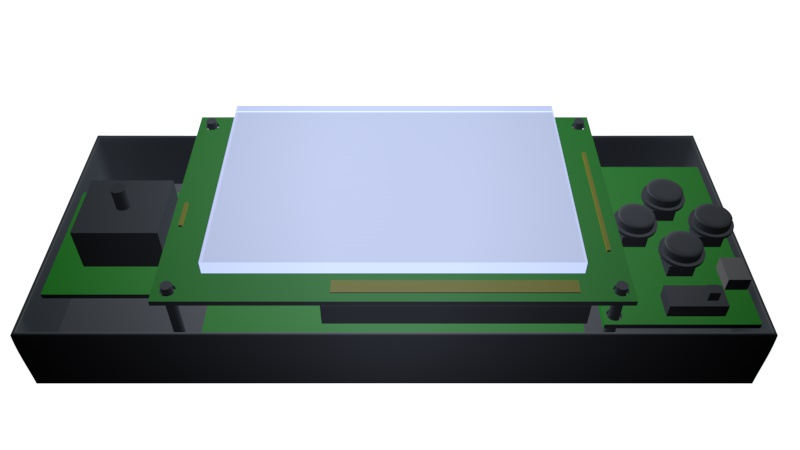
\includegraphics[width=0.7\textwidth]{bilder/studie_controller.jpg}
	\label{fig:designstudie1}
	\caption{Designstudie des Controllers}
\end{figure}

Da Junlong Yin nur noch dieses Semester bei uns ist, wurde mit Herrn Voß für ihn ein Arbeitspaket definiert, welches bis zum Ende des Semesters abzuarbeiten ist: Für die Steuerung über Neigung der Fernbedienung ist eine Weiterverarbeitung der Messwerte aus dem Beschleunigungssensor notwendig. Es wurde folgender Umfang und Ablauf seiner Arbeit definiert:
\begin{itemize}
	\item Analyse der rohen Sensorewerte hinsichtlich Rauschen (Amplitude, Spektrum) relativ zum Nutzsignal (1G in Summe aller Achsen)
	\item Entwicklung eines Modells zur Verbesserung dieser Werte (Filterung, Mittelwert, ...)
	\item Implementierung und Test dieses Modells
	\item Weiterverarbeitung der X-/Y- und Z-Sensorwerte zu Drehwinkeln in allen Achsen (trigonometrische Funktionen), die dann für die Steuerung nutzbar sind.
\end{itemize}